\documentclass[10pt,a4paper,onecolumn]{article}
\usepackage[usenames,dvipsnames]{color}
\usepackage[colorlinks,citecolor=blue]{hyperref}
\usepackage{appendix}
% we need umlauts in the refs
\usepackage[english]{babel}
\usepackage[utf8]{inputenc}
\usepackage[T1]{fontenc}

%\usepackage[natbib=true,style=authoryear,backend=biber]{biblatex}
\usepackage{authblk}
\renewcommand\Affilfont{\itshape\small}
\usepackage{graphicx}
\usepackage[authoryear]{natbib}
\usepackage{url}
\usepackage{todonotes}
%\usepackage{endfloat}
% nicer units
\usepackage{units}
% better tables
\usepackage{booktabs}
% Some colorings for the tables
%\usepackage[table]{xcolor}

%\usepackage{multirow}

% switch for final stage
%\graphicspath{{pics/}}
\graphicspath{{pics/}
              {pics/generated/}}

%\usepackage{lineno}
%\usepackage[leftbars]{changebar}
%\setlength\changebarsep{0.5em}
%\usepackage{comment}

%\usepackage[space]{grffile}
%\usepackage{latexsym}
%\usepackage{amssymb}
%\usepackage{fancyref}
\usepackage{textcomp}

\usepackage{marvosym}
\usepackage{listings}

\lstset{prebreak=\Righttorque}
\lstset{postbreak=\Lefttorque}
\lstset{breakindent=0pt}
\lstset{frame=lines}
\lstset{aboveskip=4mm}
\lstset{breaklines=true, breakatwhitespace=false}
\urlstyle{same}
% howto cite projects
\newcommand{\purl}[2]{#1\footnote{\url{#2}}}

\newcommand{\sevenT}{\unit[7]{Tesla}}
\newcommand{\threeT}{\unit[3]{Tesla}}
\newcommand{\mm}[1]{\unit[#1]{mm}}
\newcommand{\seconds}[1]{\unit[#1]{s}}

\newcommand{\ie}[0]{\emph{i.e.},\ }
\newcommand{\eg}[0]{\emph{e.g.},\ }
\newcommand{\etc}[0]{\emph{etc.}}


\begin{document}
\bibliographystyle{unsrtnat}
\title{Decoding musical genre with an fMRI encoding model of musical
features -- a 3T/7T comparison}


\author[1]{Moritz~Boos}
\author[2]{J.~Swaroop~Guntupalli}
\author[1]{Cristiano Micheli}
\author[1]{Jochem Rieger}
\author[0]{\ldots}
\author[3,4]{Michael~Hanke}

\affil[1]{Oldenburg, Germany}
\affil[2]{Department of Psychological and Brain Sciences,
  Dartmouth College, Hanover, New Hampshire, USA}
\affil[3]{Psychoinformatics lab, Department of Psychology II, University of
Magdeburg, Magdeburg, Germany}
\affil[4]{Center for Behavioral Brain Sciences, Magdeburg, Germany}
\maketitle
\thispagestyle{fancy}

\listoftodos

\begin{abstract}
% Abstracts should be up to 300 words and provide a succinct summary of the
% article. Although the abstract should explain why the article might be
% interesting, care should be taken not to inappropriately over-emphasise the
% importance of the work described in the article. Citations should not be used
% in the abstract, and the use of abbreviations should be minimized.

\todo[inline]{write abstract}
\end{abstract}

\clearpage


\section*{Introduction}

In functional magnetic resonance imaging (f{MRI}) research, voxel-wise encoding
models are an increasingly popular tool to characterize the relationship
between a real world stimulus and BOLD activity patterns
\citep{NG11,TD+06,KG+08,SZ09}.  Yet not all encoding models are made alike, and
a researcher has many degrees of freedom in constructing one.  Parameters of
the data analysis, as well as parameters of BOLD-acquisition, like field
strength and resolution, might impact encoding performance \citep{KB07,FK12}.
Especially high-field f{MRI} (7-Tesla and higher), with its increased spatial
specificity \citep{THW+05,YU08}, could lead to better encoding models \citep{FK12}. 
\citet{SF14} offer some empirical evidence that an encoding model performs better on
7-Tesla (7T) than 3-Tesla (3T) data.

After collecting the data, more choices await -- how to preprocess, which
voxels to select and how to parameterize the encoding model -- and little is known about their
consequences. Even when we obtain an encoding model for each included voxel,
we can still choose between different ways of evaluating its performance.

Previous studies have introduced several measures for the quality of
an encoding model: \citet{ML08} used a binary retrieval measure --- checking
whether an encoding model's predictions can be used to identify a stimulus from
a pair of stimuli --- to evaluate the predicted f{MRI} images for the meaning
of nouns. \citet{KG+08} used stimulus identification accuracy, and \citet{NG09} used
stimulus reconstruction quality, as a metric for encoding performance. In auditory
neuroscience, where encoding models are less frequent, only binary retrieval
accuracy \citep{CTK+2012} and stimulus identification \citep{SF14} have been
used. 

It remains an open question if these validation strategies are consistent
across different choices of analysis parameters and BOLD-acquisition schemes.

Recently, a 3T f{MRI} study on the perception of musical genres
\citep{CTK+2012} has been replicated with 7T data \citep{HDH+2015}. This makes
it possible to directly compare the effect of field strength for different 
validation strategies for encoding models. The main goal of this
study is to apply three approaches to encoding validation, binary retrieval
accuracy \citep{ML08}, stimulus identification \citep{KG+08,SF14} and
decoding accuracy of the stimulus, and compare them in a 3T
and 7T dataset with identical stimuli and comparable design, while varying
data analysis parameters.

\section*{Methods}

\subsection*{Stimuli}

Stimuli were five natural, stereo, high-quality music stimuli (\unit[6]{s}
duration; \unit[44.1]{kHz} sampling rate) for each of five different musical
genres: 1) Ambient, 2) Roots Country 3) Heavy Metal, 4) 50s Rock'n'Roll, and 5)
Symphonic. Previously, all 25 stimuli and have been made publicly available
\citep{HDH+2015}.

\subsection*{fMRI data}

The analyses presented here were performed on two independently recorded, and
previously published datasets \citep{CTK+2012,HDH+2015} . While these datasets
have been acquired using identical stimuli, with the same number of acquisition
runs and number of stimulation trials, they nevertheless differ in their
precise stimulation timing, stimulation setup and equipment, as well as other
acquisition details. A brief description of both datasets is provided below.
For more information the reader is referred to the respective publications.

\paragraph{\unit[3]{Tesla}}
%
Participants were scanned in a Philips Intera Achieva scanner with 32 channel
SENSE head coil at the Center for Cognitive Neuroscience at Dartmouth College.
Functional scans were acquired with an echo planar imaging sequence
(\unit[2]{s} TR; \unit[35]{ms} TR, \unit[90]{\textdegree} flip angle) with
\unit[3]{mm} isotropic voxels.
% MIH: as it was published before we probably don't have to include this
%All subjects consented in accordance with the procedures set by the Committee
%for the Protection of Human Subjects at the Dartmouth College. 

Each subject participated in eight functional runs. Stimuli were presented in
an event-related design with a variable trial duration. Each run consisted of a
total of 29 trials corresponding to 25 music clips and 4 catch trials presented
randomly during each run. Each trial started with a \unit[6]{s} of music clip
followed by \unit[4-8]{s} of fixation. For catch trials, a question appeared
after the audio presentation asking whether a particular feature is present in
the music clip such as vocals, guitar, etc. Subjects responded “Yes” or “No”
with a button box. Catch trials helped keep the subjects’ attention to the
music and were discarded from the analyses. Each run had \unit[4]{s} of
fixation at the beginning and \unit[10]{s} of fixation at the end. For further
details, see \citet{CTK+2012}

\paragraph{\sevenT}
%
The procedures for the \unit[7]{Tesla} acquisition were highly similar and only
criticial differences are reported here. Echo-planar BOLD images
(gradient-echo, \unit[2]{s} repetition time (TR), \unit[22]{ms} echo time,
\unit[0.78]{ms} echo spacing, GRAPPA acceleration factor 3) were acquired using
a whole-body \sevenT\ Siemens MAGNETOM magnetic resonance scanner equipped with
a 32 channel brain receive coil. 36 axial slices (thickness \unit[1.4]{mm},
\unit[1.4 $\times$ 1.4]{mm} in-plane resolution) with a 10\% inter-slice gap
were recorded in ascending order.  Slices were oriented to include the ventral
portions of frontal and occipital cortex while minimizing intersection with the
eyeballs. The field-of-view was centred on the approximate location of Heschl's
gyrus.

Instead of dedicated catch trials, similar catch questions as for the 3T
acquisition were presented \unit[4]{s} after the end of the stimulus in trials
with an \unit[8]{s} inter-stimulus delay. Consequently, each run consisted of
25 trials, and no trials were discarded from the analysis.  There was no
additional fixation at the start of a run. For further details, see
\citet{HDH+2015}, and \citet{HBI+14} for details on MRI acquisition methods.


\subsection*{Preprocessing}

Approximate temporal lobe masks for each participant were extracted from
Montreal Neurological Institute coordinate space using FSL
\citep{SJB+04,JBB+12}, and projected into the subject-specific coordinate
system.  Each voxel inside the temporal lobe mask was run-wise $Z$-scored and
linearly de-trended using PyMVPA \citep{HHS09b}. 

\begin{figure}
  \centering
  \includegraphics[width=\linewidth]{pics/encoding_scheme}

  \caption{A schematic overview of the encoding process. The spectrogram for
    each stimulus is transformed into its low-quefrency mel-frequency spectrum
    (LQ-MFS). Then, the encoding features are extracted by a sliding window
    from the LQ-MFS. Using these features, encoding model is trained on all
    runs in the training set, and used to predict the BOLD activity of the
  left-out run.  These predictions are subsequently used for validation.}

 \label{fig:encoding_scheme}
\end{figure}

\subsection*{Encoding model}

To build an encoding model with high predictive power, we need to find an
appropriate feature representation of the music stimuli.  \citet{CTK+2012}
already compared different feature representations of the same stimuli in the
3T dataset. They found features corresponding to the timbre of the
stimulus offer the best discriminative power. We chose a similar feature set made
available by \citet{HDH+2015}, the low-quefrency mel-frequency spectrum
(LQ-MFS) of the stimulus.

For each f{MRI} sample $y_{vt}$ (where $t=1,2,..,T$ denotes the time-points and
$v=1,2,..,V$ denotes the voxels) the LQ-MFS features $x_{t}$
$[1\times\widetilde{M}]$ (where $\widetilde{M}$ is the number of LQ-MFS
coefficients) of the corresponding two second part of the stimulus -- immediately
prior to the acquision time point -- were
computed. In case there was no stimulus presented at time-point $t$, a zero
vector $[1\times\widetilde{M}]$ was used. 

As the BOLD response is delayed,  the most recent feature vector was removed
for each f{MRI} sample (corresponds to an assumed \unit[2]{s} stimulus-response
delay), and the new feature vector at time-point $t$ was created by
concatenating the prior feature vectors $x_{t-1}$,$x_{t-2}$ and $x_{t-3}$ (see
Figure \ref{fig:encoding_scheme}). From now on, we denote this stacked feature
vector as $x_{t}$.  Feature vectors (and the corresponding f{MRI} sample) were
removed from the analysis, if two-thirds or more of the concatenated feature
vectors were zero-vectors.

The BOLD activity time-series, as well as the feature time-series, were
vertically stacked, resulting in a matrix of features $X$ $[N\times M]$ (where
$N$ is the number of f{MRI} samples, and $M$ is number of LQ-MFS coefficients,
with $M=3\widetilde{M}$) and a matrix of BOLD activity $Y$ $[N\times V]$ (where
$V$ is the number of voxels).

This lagging of the stimulus allows us to train the encoding model to predict
the f{MRI} time-series without explicitly modelling the BOLD response.

The encoding model could then be expressed as the probability to observe the
BOLD activity at time-point $t$ and voxel $v$:
\begin{equation}
  \label{eq:encmo}
  p(y_{vt}|x_{t}) = N(y_{vt};x_{t}\beta_{v},\sigma)
\end{equation}
where $N(y;\mu,\sigma)$ denotes the probability density at $y$ for a
Gaussian with mean $\mu$ and standard deviation $\sigma$, and $\beta_{v}$ is a
$[M\times1]$ vector of regression coefficients specific to voxel $v$. To reduce
over-fitting, the regression-coefficients were estimated using ridge regression
\citep{HK70}.  Independently for each voxel, the regularization parameter
$\lambda$ with the lowest mean squared error in a generalized leave-one-out
cross-validation \citep{GHW79} was chosen from a set of candidate values.
This set was chosen so that the highest and lowest values of $\lambda$ were only
rarely selected in cross-validation.
Later on the encoding models are validated by their predicted f{MRI} activity
for a set of voxels (visualised in the upper left corner of Figure
\ref{fig:decoding_scheme}). 


%\subsection*{Quality metrics} 
%
%
\subsubsection*{Binary retrieval accuracy}
%
Binary retrieval accuracy \citep{ML08} tests if an encoding model's predictions
can differentiate a stimulus' observed BOLD activity from the BOLD activity of
a decoy stimulus.  Specifically, a stimulus pair is counted as succesfully
classified, if the cosine similarity between predicted and observed f{MRI}
responses is greater for the correctly matched predictions and observations
than for the incorrectly matched ones (i.e. the similarity of the observed
response of stimulus A with the predictions for stimulus B and vice versa).
The binary retrieval measure for one stimulus was then computed by counting the
correct matches for all (exhaustive) pair-wise combinations of stimuli, including
stimuli from the same genre, and then dividing by the number of combinations.
This was then averaged across stimuli.


\subsubsection*{Matching score}
%
An alternative measure of encoding performance is the correlation rank score or
matching score \citep{SF14}. For each stimulus label $l_{n}$ in the validation
set, its predicted BOLD activity $\widetilde{y}_{n}$ is correlated with the
observed BOLD activity of every stimulus, $y_{i}$ for $i=1..25$. These
correlations are then ordered, and the  matching score $m(l_{n})$ is \[
m(l_{n}) = 1-\frac{rank(l_{n})-1}{N-1} \] Where $rank(l_{n})$ is the rank of
the correlation between predicted $\widetilde{y}_{n}$ and observed $y_{n}$ BOLD
activity of $l_{n}$. Finally, the matching scores for all stimuli in the
validation set are averaged.

\begin{figure}
  \centering
  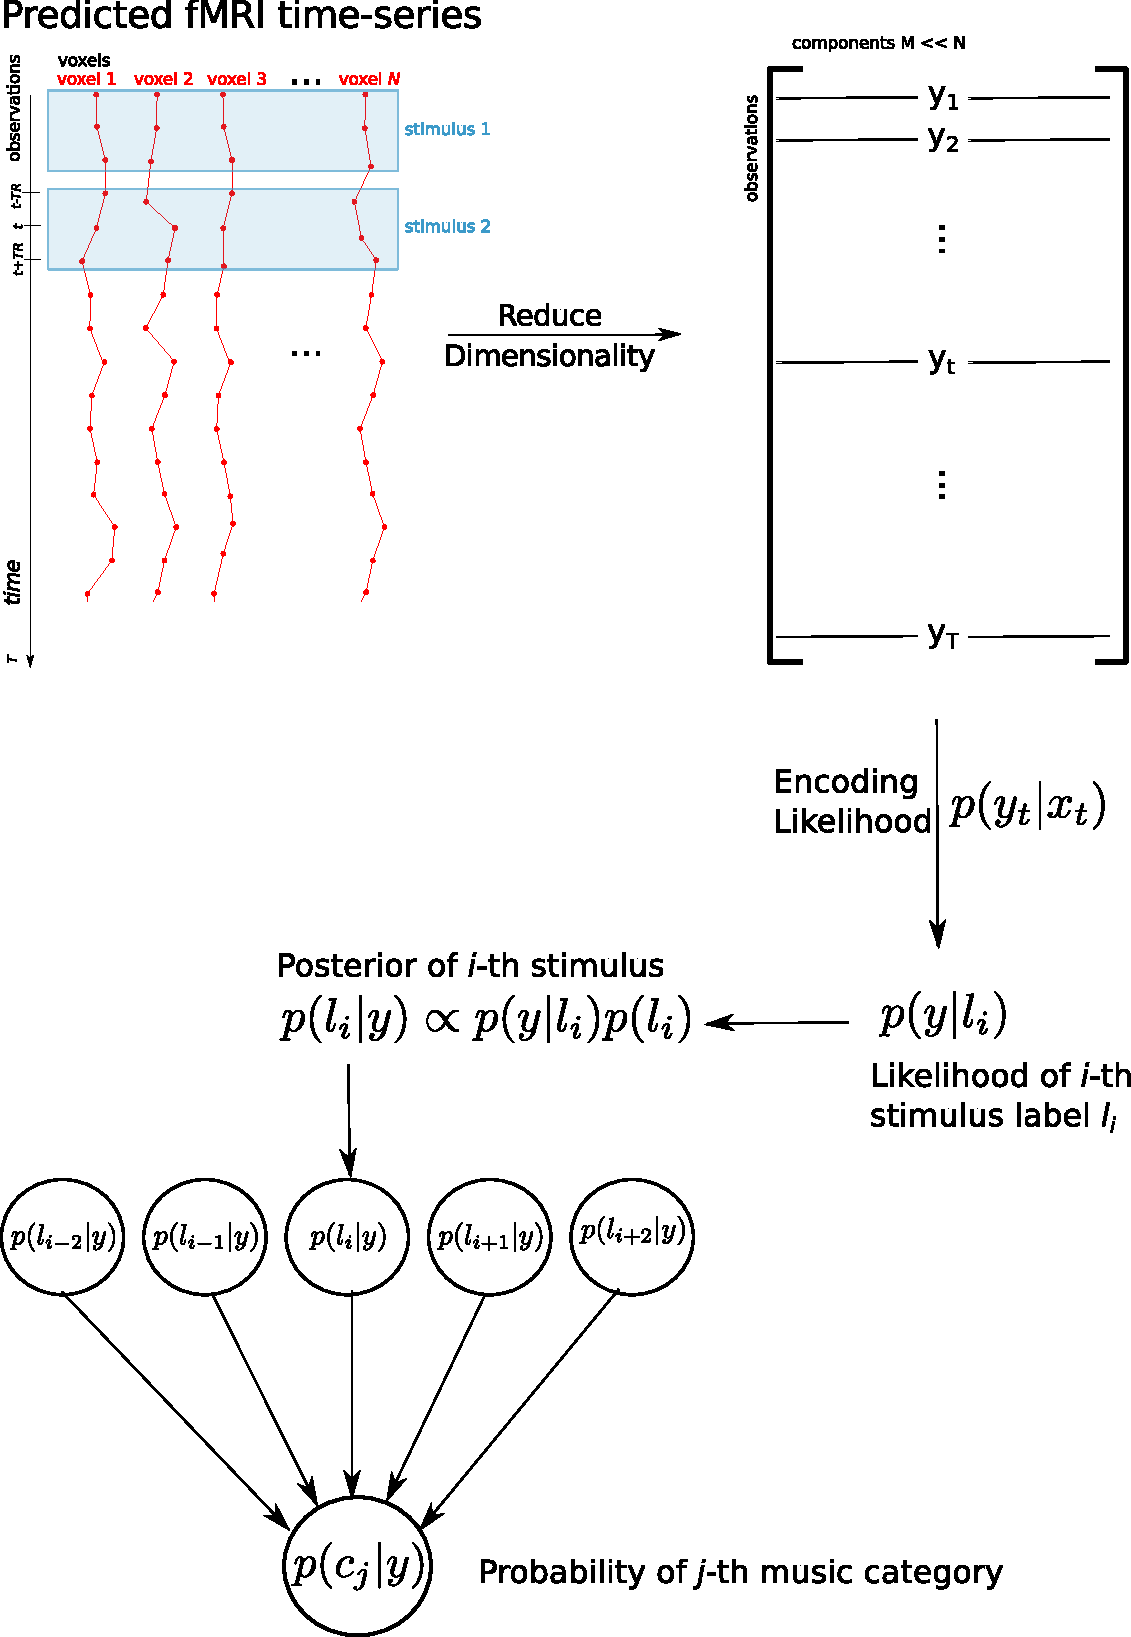
\includegraphics[width=9cm]{pics/Decoding_scheme}

  \caption{A schematic overview of the decoding of music category. The
    predicted f{MRI} time series of the validation run is reduced in
    dimensionality by principal component analysis, and a multivariate-normal
    likelihood function $p(y_{t}|x_{t})$ is constructed.  From there, the
  probability distribution over music stimuli and subsequently musical
categories is estimated.}
%\todo[inline]{this is talking about a 2-part decoding scheme. would be good to
%  label those parts. Probably best to include a symbolic reference that the
%  basic scores (without decoding) are computed from the predicted time series
%  at the top. The manuscript is unclear how models from multiple voxels are
%treated in this case. Is the correlation distance computed for all timepoints
%of a stimulus across all the voxels? or per voxel and averaged?}


 \label{fig:decoding_scheme}
\end{figure}


\subsubsection*{Decoding}

Instead of testing the encoding performance, we can also test the performance
of a decoder based on the individual encoding models \citep{NG11} (Figure
\ref{fig:decoding_scheme}).

To go from the probability of a voxel activation
given stimulus features $p(y_{vt}|x_{t})$ to probability of stimulus features
given voxel activation $p(x_{t}|y_{t})$ we follow \citet{NG09} and separate our
decoding scheme into two parts. 

\paragraph{Single- to Multi-Voxel Encoding}

First we condense the large number of voxel-specific encoding models into one
multi-voxel encoding model.  To do this we project the predicted and observed
f{MRI} data onto the first $k$ principal components of the $[N\times V]$ matrix
of predicted BOLD activity. We consider two ways of choosing $k$: using
cross-validation to estimate the number of principal components
that maximize the decoding accuracy on the training set for this participant
(1), and choosing $k$ to retain a fixed amount of variance -- 95\% -- in the
predicted BOLD activity (2). As in \citet{NG09} we construct the $k$-dimensional multivariate normal
probability density function $p(y_{t}|x_{t})$ to obtain a likelihood function
across voxels. 

\paragraph{Multi-Voxel Encoding to Decoding}

We now express this likelihood in terms of the label of the music stimulus, instead of its LQ-MFS features.  We
use the simplifying assumption that the BOLD activity is influenced by the
music stimuli only through their LQ-MFS coefficients $x$, and --- given that
each music stimulus was associated with only three (lagged) LQ-MFS
representations --- the likelihood to observe a given triple of consecutive $y$
for a specific music stimulus $l_{i}$ is $p(y|l_{i}) \propto
p(y_{t-1}|x_{1})p(y_{t}|x_{2})p(y_{t+1}|x_{3})$ where $t$ is the sample 6
seconds after the start of the music stimulus and $x$ are the three LQ-MFS
feature vectors of this stimulus.  For a given triple of consecutive BOLD
activity $y$ from the same stimulus, we can now estimate the probability
distribution over music stimuli $p(l_{i}|y)$ (for $i=1..25$) by using Bayes'
rule: $p(l_{i}|y) \propto p(y|l_{i})p(l_{i})$.
Since each stimulus was presented was presented exactly once,
it has an uniform prior distribution with $p(l_{i})=\frac{1}{25}$. The mode of
this distribution is the most probable presented stimulus given the data. 
Additionally we can decode the musical genre of the presented stimulus given the observed
BOLD activity as the mode of $p(c_{i}|y) = \sum\nolimits_{l \in
  stim(c_{i})} p(l|y)$ where $stim(c_{i})$ are the labels of the stimuli
  belonging to the genre $c_{i}$. 


\subsection*{Voxel selection}

We varied the number of voxels used in the analysis, both for 3T and 7T
f{MRI} data, and selected which voxels to keep by two different criteria. Both
criteria were based on voxel characteristics in the training set only.

\paragraph{Selection by stability}

\citet{ML08} selected the 500 most stable voxels for their analysis. For a
single voxel, each run can be represented as a vector of BOLD activity, where
each entry is associated with one stimulus. A voxel's "stability score" is then
the average (pair-wise) correlation between the vectors of the eight runs for
all combinations of runs.  This criterion selects voxels with consistent
activation for each stimulus across runs.

\paragraph{Selection by $r^2$}

As we are interested in encoding performance, we can use the quality of
predictions of each voxel's encoding model as a selection criterion. We compute
the coefficient of determination $r^2$ for each voxel-specific encoding model
in the training set. Using this criterion selects voxels whose activity can be
explained best by an LQ-MFS-based encoding model.

\section*{Results}

We varied the number of voxels used in the analysis and how they were selected,
both for 3T and 7T f{MRI} data, and compared the resulting differences in
three encoding metrics. To differentiate between effects of voxel number and
overall volume of the voxels, which differs in 3T and 7T, we show the
results as a function of the number of voxels, as well as overall volume of
these voxels.

\begin{figure}
  \centering
  \def\svgwidth{\linewidth}
  \input{pics/binary_score_joint.pdf_tex}
	
  \caption{\textbf{A} Mean binary retrieval accuracy as a function of the
  included number of voxels for 3T and 7T, for stability- and $r^2$-based
  voxel selection. Error bars denote the bootstrapped 95\% confidence interval
  of the mean. The mean is taken over binary retrieval accuracies of eight runs
  for each of the 19 participants. \textbf{B} Mean binary retrieval accuracy as
a function of the overall volume of the included voxels for 3T and 7T, for
stability- and $r^2$-based voxel selection.
}

 \label{fig:binary_retrieval}
\end{figure}

\subsection*{Binary retrieval accuracy}

Differences in binary retrieval accuracy are shown in Figure
\ref{fig:binary_retrieval}. For the stability selection criterion, binary retrieval
accuracy is higher in 3T than 7T data for lower numbers of voxels.
When a higher number of the most stable voxels are included, binary retrieval
accuracy increases for 7T data, while decreasing for 3T data. In
contrast, increasing the number of voxels included by $r^2$ decreases the
binary retrieval accuracy for 3T, as well as 7T data, although the
decrease seen in 3T data is larger. Indexing by the overall volume of the voxels, reveals a very similar,
but shifted, pattern for 3T and 7T data.

\begin{figure}
  \centering
  \def\svgwidth{\linewidth}
  \input{pics/matching_score_joint.pdf_tex}
	
  \caption{\textbf{A} Mean matching score as a function of the included number
  of voxels for 3T and 7T, for stability- and $r^2$-based voxel selection.
  Error bars denote the bootstrapped 95\% confidence interval of the mean. The
  mean is taken over binary retrieval accuracies of eight runs for each of the
  19 participants. \textbf{B} Mean matching score as a function of the overall
volume of the included voxels for 3T and 7T, for stability- and
$r^2$-based voxel selection.}

 \label{fig:matching_score}
\end{figure}

\subsection*{Matching score}

Figure \ref{fig:matching_score} shows the matching score. Again, for few
voxels, encoding models for 3T data produce a higher score than encoding
models for 7T data. Increasing the number of voxels increases the matching
score for 7T data, and decreases the score for 3T data. This pattern
is present in both selection criteria. For voxels selected by $r^2$, there is a
steeper increase and decrease and a higher peak for both field strengths.  If
indexed by the overall voxel volume, similarities in the overlapping regions of
the 3T and 7T matching score curves can be seen.


\begin{figure}
  \centering
  \def\svgwidth{\linewidth}
  \input{pics/Stimulus_decoding.pdf_tex}
	
  \caption{ Decoding of the stimulus itself with dimensionality chosen so it
	  retains 95\% of variance }%\todo[inline]{extend y-axis to include 0.04 as chance level?} }

 \label{fig:decoding_accuracy_stimulus}
\end{figure}

\begin{figure}
  \centering
  \def\svgwidth{\linewidth}
  \input{pics/Category_decoding_var95.pdf_tex}
	
  \caption{ Decoding accuracy now with the number of eigenvectors chosen to
  retain 95\% of the variance instead of cross-validated for decoding }

 \label{fig:decoding_accuracy_var95}
\end{figure}

\begin{figure}
  \centering
  \def\svgwidth{\linewidth}
  \input{pics/Category_decoding_cv.pdf_tex}
	
  \caption{\textbf{A} Mean decoding accuracy of music category as a function of
  the included number of voxels for 3T and 7T, for stability- and
  $r^2$-based voxel selection. Error bars denote the bootstrapped 95\%
  confidence interval of the mean. The mean is taken over decoding
  accuracies of eight runs for each of the 19 participants. \textbf{B} Mean
decoding accuracy of music category as a function of the overall volume of the
included voxels for 3T and 7T, for stability- and $r^2$-based voxel
selection.
}

 \label{fig:decoding_accuracy}
\end{figure}

\begin{figure}
  \centering
  \def\svgwidth{\linewidth}
  \input{pics/confusion_matrices.pdf_tex}
	
  \caption{ Confusion matrices for genre decoding, separated by field-strength
  and voxel selection. Each confusion matrix is averaged across the different number
  of voxels, participants and runs, for each cell the mean and standard deviation (in parentheses)
  are given. }

 \label{fig:confusion_matrices}
\end{figure}

\subsection*{Decoding accuracy}

Figure \ref{fig:decoding_accuracy_stimulus} shows the accuracy of decoding each
individual stimulus. We compare the performance of our encoding-based decoder
with a linear Support Vector Classifier (SVC) \citep{FCH+08,V13} that predicts
stimulus labels using the time series from the selected voxels (dashed lines).
While such a decoder can use the subset of the most stable
voxels, it can only select the voxels with the highest $r^2$ if it can access
the information from an encoding model. We still include these data, to show
which information could be extracted from these voxels by a more sophisticated
decoding approach. 

Decoding accuracy for the most stable voxels is slightly higher in 3T than 7T
data, and similar across different numbers of voxels. For voxels selected by
$r^2$, 3T shows a higher decoding accuracy than 7T for fewer voxels, and
a similar performance if the number of voxels increases.
Independent from voxel number and selection, support vector classification
performs worse than the encoding-based decoder.

The decoding accuracy of each stimulus's music category is shown in Figure
\ref{fig:decoding_accuracy_var95}.  The decoding accuracy was higher for 7T data than for
3T data, across all voxel numbers and selection criteria. 7T decoding
accuracy increases with the number of most stable voxels, while 3T stays level.
For voxels selected by $r^2$, 7T decoding accuracy peaks around 2500 voxels,
then decreases, while 3T decreases in decoding accuracy from 500 voxels
on. 


Instead of reducing the dimensionality of the encoding model to retain a fixed
amount of variance, we wanted to see if choosing the dimensionality to optimise decoding
performance affects the genre decoding accuracy.
Figure \ref{fig:decoding_accuracy} shows these results, note that the support vector
classification curves stay the same and can be used as a reference point.
Both 7T and 3T show a higher decoding accuracy and better performance especially
for lower numbers of voxels. 

Overall decoding accuracy can be complemented by the confusion matrix of a
classifier: Rows are annotated by the true class label, columns by the
classifier's chosen class label. Each cell contains the count -- or proportion
-- of occurences of this row/column combination. A perfect classification
accuracy, implies a diagonal confusion matrix.

In Figure \ref{fig:confusion_matrices} the confusion matrices averaged across
numbers of voxels for different field strength and selection criteria are shown.
The occurences are normalized per row, and their mean proportion together with
the standard deviation across numbers of voxels are indicated in each cell. All
confusion matrices show a higher misclassification between genres that contain
speech (country, rock'n'roll and heavy metal) and between instrumental genres
(ambient and symphonic), while very few genres that contain speech are
incorrectly classified as instrumental or vice versa.

\begin{figure}
  \centering
  \def\svgwidth{\linewidth}
  \input{pics/r2_means.pdf_tex}
	
  \caption{ Mean $r^2$ of voxels sorted by $r^2$.}

 \label{fig:r2}
\end{figure}

\begin{figure}
  \centering
  \def\svgwidth{\linewidth}
  \input{pics/Mean_fstatistic_stim_cat.pdf_tex}
	
  \caption{ Mean voxel-wise F-statistic for the f{MRI} time series averaged over
  the voxels selected by $r^2$ for genre or stimulus.}

 \label{fig:anova}
\end{figure}

\begin{figure}
  \centering
  \def\svgwidth{\linewidth}
  \input{pics/Mean_fstatistic_stim_cat_yhat.pdf_tex}
	
  \caption{ Mean voxel-wise F-statistic for the predicted f{MRI} time series averaged over
  the voxels selected by $r^2$ for genre or stimulus.}

 \label{fig:anova_yhat}
\end{figure}


\subsection*{Voxel-wise $r^2$ and discriminability}
%
Instead of validating encoding performance for a set of voxels, we can also test
each voxel independently.

To quantify each voxel's encoding performance -- in terms of explained
variance -- with the discriminability of the selected voxels, we order each
participant's voxels by explained variance and compute the mean $r^2$ for each
voxel across participants (Figure \ref{fig:r2}). Vertical bars the point up to
which voxels were selected by $r^2$. 

The potential discriminability of a voxel can be illustrated by computing its
F-statistic. This measure is the between-group variability divided by the within-group
variability, where the groups are either the stimulus or genre labels. 
Additionally, we can then test if an encoding model actually increases the
discriminability, by computing this measure for the original f{MRI} time-series as well
as the time-series predicted by the voxel-wise encoding models. In Figure
\ref{fig:anova} we show the F-statistic first averaged over the
voxels selected by $r^2$ and then averaged over participants, for the original
time series (left column) and for the time series predicted by an encoding model
(right column).

Grouping the observed f{MRI} time-series both by genre and stimuli shows a
higher F-statistic for 7T than 3T across all numbers of voxels, with an
especially strong difference for grouping by genre.

Using the predicted f{MRI} time-series increases the discriminability overall,
with the largest difference again for genre.

\section*{Discussion}

Our results show considerable variation of different quality metrics with
field strength and parameters of the data analysis. We demonstrate that the
patterns of this variation differ between validation strategies and that the
effects of field strength, voxel selection, and voxel number are inconsistent
across these metrics.

Specifically, we show a similar performance in purely encoding based metrics
for 3T and 7T data with a slightly worse peak performance for 7T, but
observe that this effect is mediated by the number of voxels used. A previous
study \citep{SF14} found a better performance for 7T data for the matching
score, although using a different number of stimuli in the 3T and 7T
datasets. 

Selecting the voxels by $r^2$ instead of a stability criterion, improves
performance especially in the lower number of voxels for the binary retrieval
accuracy and the decoding accuracy, while widening the performance gap between
3T and 7T data in the matching score. Including voxels ordered by $r^2$
--- a measure that captures encoding performance in a single voxel --- gives
diminishing returns for higher numbers of voxels: Voxels for which an encoding
model performs well are already included, and each additional voxel decreases
the joint encoding performance.  Interestingly, this pattern is not seen in the
matching score, where performance in 7T is worse for the smallest number
of voxels and increases with voxel number. The same pattern is seen in the
performance of the linear SVC. Even with information from an encoding model ---
selecting voxels by $r^2$ --- a standard decoder can initially not take
advantage of this information as well as an encoding model. For the high field
strength condition, the decoder improves if more voxels are included and
eventually performs better than the encoding model. This might be an effect of
the sheer number of features used by the decoder, or of the information content
of these voxels, i.e. because the decoder profits from pattern information that
is not related to the LQ-MFS features of the stimulus, and would therefore be
more present in a voxel with lower $r^2$ in encoding LQ-MFS.

The number of voxels affect the encoding performance differentially for low and
high field strength. This is not surprising, as voxel sizes differ for these
particular 3T and 7T data. Indexing by the overall volume of the selected
voxels, instead of their number, reveals similarities in performance when 3T
and 7T encoding models are trained on a similar volume in the matching
score, but other metrics show a higher sensitivity to the number of
voxels.

All quality metrics show a different pattern for field strength differences.
One might expect a better encoding performance in 7T than 3T a priori, since 7T contains
potentially higher information \citep{FK12}, but only in decoding the music genre
is there a consistently higher performance for 7T data.

Training encoding models on stimulus features makes stimulus labels as the
boundaries of f{MRI} activity somewhat arbitrary. Two stimuli might be quite
similar, and the encoding model might correctly translate this into similar BOLD
activity, but this could still decrease a quality measure that is based on the
correct discrimination between individual stimuli. We also observe this in our
study: In 7T there's a higher voxel-wise explained variance (Figure \ref{fig:r2}) and a higher potential discriminability
between stimuli and genre (Figure \ref{fig:anova} and \ref{fig:anova_yhat}). Yet, this difference does not translate into a higher
binary retrieval accuracy, matching score or stimulus decoding accuracy. Only
in decoding information about the similarity between stimuli -- their genre
-- is there an advantage of the better voxel-wise encoding models present in
7T.

Which validation strategy should one then choose?

Selecting voxels by $r^2$ outperforms a stability-based selection consistently.
If this information is available, it should be used. It helps
discriminating stimuli using fewer voxels, and it is more justified to interpret
the location of voxels selected by $r^2$ than by a stability criterion.
Voxels can alternatively be selected by anatomical criteria.

Different numbers of voxels interact with different quality metrics and they
have to be considered together. 

Binary retrieval accuracy shows the highest similarity between 3T and 7T data
across different numbers of voxels, the effect of the number of voxels is
stronger than their volume. The matching score on the other hand shows
sensitivity to the overall volume of the selected voxels, potentially indicating
the size of the region(s) in the temporal lobe where the signal is strongest.

By considering only the pair-wise similarity, the binary retrieval score is a more stable measure than the matching
score or the decoding accuracy, but that stability comes with a price: The measure
quickly saturates and it might become difficult to detect performance
differences for well performing models. The matching score ranks one
stimulus's prediction against all stimuli, and more accurately represents how
well stimuli can be discriminated. Decoding the stimulus identity through an
encoding model does this as well, but adds an additional degree of freedom: how to select the dimensionality
of the reduced encoding model. Yet, using a encoding-based  decoder also has an
advantage over the matching score. It is not limited to decoding the
stimulus identity, but can be used to decode other stimulus features -- like its
genre -- which might capture similarity between stimuli, or their associated
f{MRI} response, better. The decoding approach might better capture the individual voxel-wise encoding
model's performance if the set of stimuli can be separated by other labels than the stimulus identity.

Yet, the main take-away of this study might be a different one: Arbitrary
choices in the data analysis, -- like the number of voxels used or how they are
selected -- have a considerable impact on the performance evaluation of
voxel-wise encoding models. Even worse, the impact of these parameters is vastly
different for the considered validation strategies. The effects of these
hyper-parameters are rarely known, and each choice of a specific value can
easily be justified, but there are considerable researcher degrees-of-freedom
\citep{SNS11} in arriving at the end-result.

\section*{Author contributions}
%In order to give appropriate credit to each author of an article, the
%individual contributions of each author to the manuscript should be detailed
%in this section. We recommend using author initials and then stating briefly
%how they contributed.

MB performed the analysis and wrote the manuscript.
JSG contributed to the manuscript.
MH contributed to the manuscript.
\todo{some authors are missing here}


\section*{Competing Interests}

No competing interests were disclosed.

\section*{Grant Information}

This research was, in part, supported by the German Federal Ministry of
Education and Research (BMBF) as part of a US-German collaboration in
computational neuroscience (CRCNS; awarded to James Haxby, Peter Ramadge, and
Michael Hanke), co-funded by the BMBF and the US National Science Foundation
(BMBF 01GQ1112; NSF 1129855).  Work on the data-sharing technology employed for
this research was supported by US-German CRCNS project awarded to
Yaroslav~O.~Halchenko and Michael~Hanke, co-funded by the BMBF and the US
National Science Foundation (BMBF 01GQ1411; NSF 1429999).  Michael Hanke was
supported by funds from the German federal state of Saxony-Anhalt, Project:
Center for Behavioral Brain Sciences.


\section*{Acknowledgements}
%This section should acknowledge anyone who contributed to the research or the
%article but who does not qualify as an author based on the criteria provided
%earlier (e.g. someone or an organisation that provided writing assistance).
%Please state how they contributed; authors should obtain permission to
%acknowledge from all those mentioned in the Acknowledgements section.  Please
%do not list grant funding in this section (this should be included in the
%Grant information section - See above).

We are grateful to Michael Casey and the musicians ;) \ldots
\todo{move Michael into the author list, if he agrees}

\todo[inline]{express gratitude}

\bibliography{references}
\end{document}

% vim: textwidth=80 colorcolumn=81
